
% Tento soubor slouží jako šablona/příklad pro generování protokolu

\documentclass{protokol}

%====== Vyplňte údaje ======
\jmeno{David Strašák}
\kod{219502}
\rocnik{3.}
\obor{MET}
% \skupina{3.}
% \spolupracoval{Šimon Pokorný, Bence Simonics}

\merenodne{06.\,03.\,2025}
\odevzdanodne{07\,.03.\,2025}

\nazev{Provedení zkoušek nakrátko a naprázdno na neznámém transformátoru}
% \cislo{99} %měřené úlohy

\predmet{Elektromechanická přeměna energie}
\ustav{UVEE, FEKT VUT v Brně}
% \skola{FEKT VUT v Brně}
%%%%%%%%%%%%%%%%%%%%%%%%%%%%%%%%%%%%%%%%%%%%%%%%%%%%%%%%%%%%%%%%%%%%%%%%%%%%%%%%%%%%%%%%%%%%%%%%%%%%%%%%%%%%%%%%%%%%%%%%%%%%%%%%%%%%%%%%%%%%%%%%%%%%%%%%%%%%%%%%%%%%%%%%%%%%%%%%%%%%%%%%%%%%%%%%%%%%%%%%%%%%%%%%%%%%
\begin{document}
%====== Vygenerování tabulky ======
\maketitle
%====== Úvodní texty protokolu ======

\section{Zadání}
\begin{enumerate}
    \item Voltampérovou metodou změřte odpory všech vinutí.
    \item Změřte převod transformátoru.
    \item Proveďte měření nakrátko.
    \item Proveďte měření naprázdno.
    \item Vypočítejte procentní proud naprázdno a procentní napětí nakrátko.
    \item Určete velikosti prvků náhradního schématu transformátoru přepočtené na primární i na sekundární stranu.
    \item Nakreslete dvě náhradní schémata, do jednoho vepište velikosti prvků přepočtené na primární stranu, do druhého na sekundární.
    \item Zhodnoťte měření.
\end{enumerate}

%%%%%%%%%%%%%%%%%%%%%%%%%%%%%%%%%%%%%%%%%%%%%%%%%%%%%%%%%%%%%%%%%%%%%%%%%%%%%%%%%%%%%%%%%%%%%%%%%%%%%%%%%%%%%%%%%%%%%%%%%%%%%%%%%%%%%%%%%%%%%%%%%%%%%%%%%%%%%%%%%%%%%%%%%%%%%%%%%%%%%%%%%%%%%%%%%%%%%%%%%%%%%%%%%%%%
\section{Teoretický rozbor}
Transformátor je netočivý elektrický stroj, který převádí elektrickou energii na elektrickou energii pomocí elektromagnetické indukce. Transformace je provedena na základě přeměny elektrické energie do magnetické a naopak, díky čemuž je transformátor schopný měnit napětí elektřiny, kterou do něj vkládám. Změna napětí je určena převodem transformátoru. 

V naše případě se jednalo o transformátor třífázový. Na tomhle transformátoru je možné ho zapojit do jakékoliv konfigurace s jakýmkoliv hodinovým úhlem. Zadáním ale bylo zapojení Yy0. Spojení do hvězdy se provádí tak, že se všechny konce na vnitřních stranách všech fází spojí na stejný potenciál.

\begin{figure}[H]
    \centering
    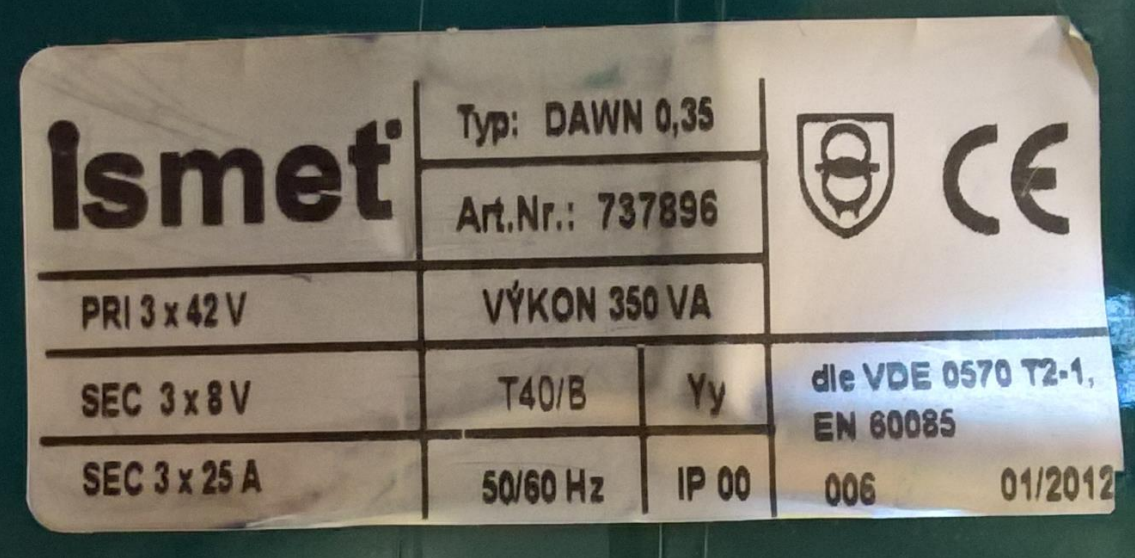
\includegraphics[width=0.8\linewidth]{TrafoStitek.png}
    \caption{Štítek měřeného transformátoru}
    \label{fig:TrafoStitek}
\end{figure}

%%%%%%%%%%%%%%%%%%%%%%%%%%%%%%%%%%%%%%%%%%%%%%%%%%%%%%%%%%%%%%%%%%%%%%%%%%%%%%%%%%%%%%%%%%%%%%%%%%%%%%%%%%%%%%%%%%%%%%%%%%%%%%%%%%%%%%%%%%%%%%%%%%%%%%%%%%%%%%%%%%%%%%%%%%%%%%%%%%%%%%%%%%%%%%%%%%%%%%%%%%%%%%%%%%%%
\section{Voltampérovou metodou změřte odpory všech vinutí}
V rámci tohoto úkolu bylo cílem pomocí generátoru stejnosměrného napětí změřit odpor vinutí na jednotlivých fázích transformátoru. 

Postup který byl zvolen v rámci tohoto měření bylo přivést na 1 fázi transformátoru stejnosměrné napětí a změřit napětí a proud na fázi. Následně je pomocí Ohmova zákona možné dopočítat odpor fáze.
\begin{equation}
    R = \frac{U}{I}    
    \label{eq:OhmuvZakon}
\end{equation}

\begin{figure}[H]
    \centering
    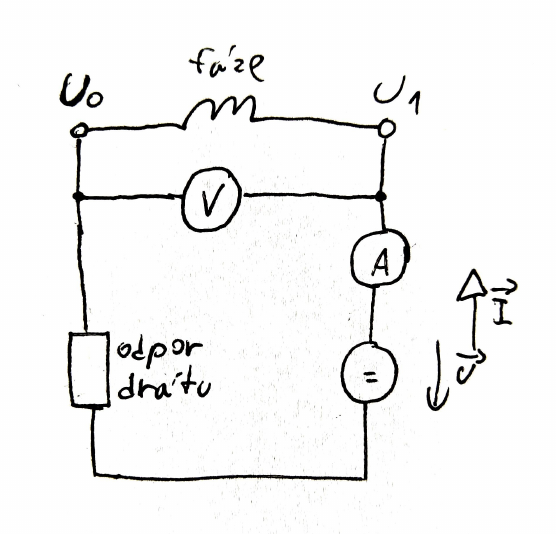
\includegraphics[width=0.5\linewidth]{MereniOdporuNaJedneFazi.png}
    \caption{Měření odporu na jedné fázi}
    \label{fig:MereniOdporu}
\end{figure}

% Please add the following required packages to your document preamble:
% \usepackage[table,xcdraw]{xcolor}
% Beamer presentation requires \usepackage{colortbl} instead of \usepackage[table,xcdraw]{xcolor}
\begin{table}[H]
\centering
\caption{Měření odporů vinutí transformátoru}
\begin{tabular}{lrrr}
\rowcolor[HTML]{F8F9FA} 
Měření & \multicolumn{1}{l}{\cellcolor[HTML]{F8F9FA}U1{[}V{]}} & \multicolumn{1}{l}{\cellcolor[HTML]{F8F9FA}I1{[}A{]}} & \multicolumn{1}{l}{\cellcolor[HTML]{F8F9FA}Odpor{[}Ohm{]}} \\
\cellcolor[HTML]{FFFFFF}U & \cellcolor[HTML]{FFFFFF}0.722 & 5.268 & 0.137 \\
V & 0.721 & 5.292 & 0.136 \\
W & 0.721 & 5.284 & 0.136 \\
u & 0.272 & 21.923 & 0.012 \\
v & 0.265 & 22.102 & 0.012 \\
w & 0.265 & 22.047 & 0.012
\end{tabular}
\label{tab:MereniOdporuVinuti}
\end{table}

Z tohoto měření vychází průměrné hodnoty odporů vinutí:
\begin{itemize}
    \item $R_{primar} = 136 m\Omega$
    \item $R_{sekundar} = 12 m\Omega$
\end{itemize}

%%%%%%%%%%%%%%%%%%%%%%%%%%%%%%%%%%%%%%%%%%%%%%%%%%%%%%%%%%%%%%%%%%%%%%%%%%%%%%%%%%%%%%%%%%%%%%%%%%%%%%%%%%%%%%%%%%%%%%%%%%%%%%%%%%%%%%%%%%%%%%%%%%%%%%%%%%%%%%%%%%%%%%%%%%%%%%%%%%%%%%%%%%%%%%%%%%%%%%%%%%%%%%%%%%%%
\section{Změřte převod transformátoru}
Změřit převod transformátoru je možné tím, že se zároveň měří napětí na jedné fázi primáru a zároveň na stejné fázi sekundáru. Během měření převodu by mělo být na primáru nastavené jmenovité fázové napětí.

Vzhledem k tomu, že měříme fázové napětí, je nejdříve nutné přepočítat jmenovité napětí na fázové. Fázové napětí se z jmenovitého vypočítá tímto způsobem:

\begin{equation}
    U1f = \frac{U1}{\sqrt{3}} = \frac{42}{\sqrt{3}} = 24,25 V
    \label{eq:PrevodNominalnihoNapetiNaFazove}
\end{equation}

\begin{table}[H]
\centering
\caption{Hodnoty naměřené na primárním a sekundárním vinutí transformátoru}
\begin{tabular}{ll}
\rowcolor[HTML]{F8F9FA} 
U1[V]& U2[V] \\
\rowcolor[HTML]{FFFFFF} 
\multicolumn{1}{r}{\cellcolor[HTML]{FFFFFF}24.233} & \multicolumn{1}{r}{\cellcolor[HTML]{FFFFFF}4.955}
\end{tabular}
\label{tab:NamereniNapetiNaPrimaruASekundaru}
\end{table}

Z těchto hodnot je možné vypočítat převod transformátoru pomocí tohoto vzorce:
\begin{equation}
    k = \frac{U1f}{U2f} = \frac{24.233}{4.955} = 4.891
    \label{eq:VypocetPrevoduTransformatoru}
\end{equation}

%%%%%%%%%%%%%%%%%%%%%%%%%%%%%%%%%%%%%%%%%%%%%%%%%%%%%%%%%%%%%%%%%%%%%%%%%%%%%%%%%%%%%%%%%%%%%%%%%%%%%%%%%%%%%%%%%%%%%%%%%%%%%%%%%%%%%%%%%%%%%%%%%%%%%%%%%%%%%%%%%%%%%%%%%%%%%%%%%%%%%%%%%%%%%%%%%%%%%%%%%%%%%%%%%%%%
\section{Proveďte měření}
Při obou měření je zapojení transformátoru i zapojení měřících sond stejné, ale mění se strana, kde jsou sondy zapojeny. 

Zapojení je vždy do hvězdy a tak jsou vždy spojené potenciály z vnitřních tran vinutí. Specificky jsou tedy v obou měřeních spojené vstupy na primáru: U0, V0, W0 a vstupy na sekundáru: u0, v0 a w0.

Napětí, které měříme je napětí svorkové a tak bude vždy před počítáním potřebné si zkontrolovat, že počítáme s fázovým napětím, které je pro Yy0 transformátor vždy o $\sqrt{3}$ menší než napětí svorkové.
\begin{figure}[H]
    \centering
    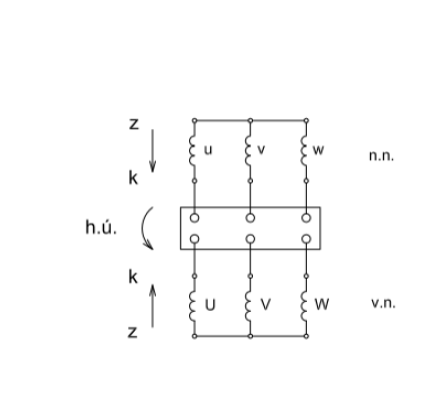
\includegraphics[width=0.5\linewidth]{ZapojeniDoHvezdy.png}
    \caption{Zapojení transformátoru do hvězdy}
    \label{fig:ZapojeniDoHvezdy}
\end{figure}

Měřící sondy byly zapojeny za základě následujícího obrázku:

\begin{figure}[H]
    \centering
    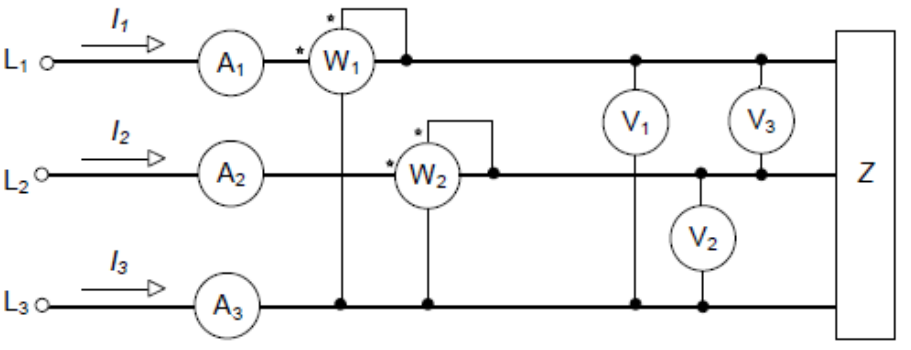
\includegraphics[width=0.5\linewidth]{ZapojeniMeraku.png}
    \caption{Zapojení při měření naprázdno}
    \label{fig:ZapojeniMeraku}
\end{figure}

Díky tomuto zapojení měřících sond máme z měření přímo informaci o činném výkonu transformátoru a navíc všechny informace o svorkových napětích a proudech na primáru a sekundáru. Z toho je možné vzít průměrné hodnoty napětí a proudu na vinutích a s nimi spočítat hodnoty prvků náhradního schématu.

%%%%%%%%%%%%%%%%%%%%%%%%%%%%%%%%%%%%%%%%%%%%%%%%%%%%%%%%%%%%%%%%%%%%%%%%%%%%%%%%%%%%%%%%%%%%%%%%%%%%%%%%%%%%%%%%%%%%%%%%%%%%%%%%%%%%%%%%%%%%%%%%%%%%%%%%%%%%%%%%%%%%%%%%%%%%%%%%%%%%%%%%%%%%%%%%%%%%%%%%%%%%%%%%%%%%
\subsection{Měření nakrátko}
Měření nakrátko je prováděno na primáru. Měřící sondy jsou zapojeny na bodech U1, V1 a W1. Tyto fáze jsou zapojeny vždy postupně na vodičích, které v obrázku \ref{fig:ZapojeniMeraku} vedou dovnitř impedance na pravé straně.

Pro tohle měření je potřeba si určit proud, který by měl být naměřený. Při zkoušce nakrátko by mělo jít o jmenovitý proud a ten se dá dopočítat z celkového zdánlivého výkonu transformátoru:

\begin{equation}
    I_{1f} = I_{1} = \frac{S}{U1*\sqrt{3}} = \frac{350}{42*\sqrt{3}} = 4.811 A
    \label{eq:VypocetProuduZVykonu}
\end{equation}

Při měření se tedy postupovalo tak, že se zvyšovalo napětí na autotransformátoru dokud nebyl průměr všech proudů přibližně rovný této hodnotě. 

Zde jsou výsledky tohoto měření: 
\begin{table}[H]
\centering
\caption{Výsledky měření nakrátko}
\label{tab:MereniNakratko}
\begin{tabular}{lllllllll}
\rowcolor[HTML]{F8F9FA} 
U1{[}V{]} & U2{[}V{]} & U3{[}V{]} & U0{[}V{]} & I1{[}A{]} & I2{[}A{]} & I3{[}A{]} & I0{[}A{]} & P0{[}W{]} \\
\rowcolor[HTML]{FFFFFF} 
\multicolumn{1}{r}{\cellcolor[HTML]{FFFFFF}4.820} & \multicolumn{1}{r}{\cellcolor[HTML]{FFFFFF}4.909} & \multicolumn{1}{r}{\cellcolor[HTML]{FFFFFF}4.931} & \multicolumn{1}{r}{\cellcolor[HTML]{FFFFFF}4.886} & \multicolumn{1}{r}{\cellcolor[HTML]{FFFFFF}4.729} & \multicolumn{1}{r}{\cellcolor[HTML]{FFFFFF}4.824} & \multicolumn{1}{r}{\cellcolor[HTML]{FFFFFF}4.707} & \multicolumn{1}{r}{\cellcolor[HTML]{FFFFFF}4.753} & \multicolumn{1}{r}{\cellcolor[HTML]{FFFFFF}40.122}
\end{tabular}
\end{table}

Jelikož transformátor není perfektně symetrický, vznikají na různých fázích různé úbytky napětí. Proto je dobré pro naše výpočety později používat pouze hodnoty U0, I0 a P0, protože tyhle hodnoty již jsou aritmeticky zprůměrované. 

%%%%%%%%%%%%%%%%%%%%%%%%%%%%%%%%%%%%%%%%%%%%%%%%%%%%%%%%%%%%%%%%%%%%%%%%%%%%%%%%%%%%%%%%%%%%%%%%%%%%%%%%%%%%%%%%%%%%%%%%%%%%%%%%%%%%%%%%%%%%%%%%%%%%%%%%%%%%%%%%%%%%%%%%%%%%%%%%%%%%%%%%%%%%%%%%%%%%%%%%%%%%%%%%%%%%
\subsection{Měření naprázdno}
Měření naprázdno je prováděno na sekundáru. Měřící sondy jsou zapojeny na bodech u1, v1 a w1. Tyto fáze jsou zapojeny na vodičích, které v obrázku \ref{fig:ZapojeniMeraku} vedou dovnitř impedance na pravé straně.

Pro tohle měření je potřeba nastavit na měřícím zařízení nominální napětí na sekundáru, které je 8V. Měřící sondy jsou zapojeny tak, aby měřili svorkové napětí, které je zároveň dané nominální napětí.

Při měření se postupovalo tak, že se zvyšovalo napětí na autotransformátoru dokud nebyl průměr všech napětí U0 rovný chtěné hodnotě.

Zde jsou výsledky tohoto měření:
\begin{table}[H]
\centering
\caption{Výsledky měření naprázdno}
\label{tab:MereniNaprazdno}
\begin{tabular}{lllllllll}
\rowcolor[HTML]{F8F9FA} 
U1{[}V{]} & U2{[}V{]} & U3{[}V{]} & U0{[}V{]} & I1{[}A{]} & I2{[}A{]} & I3{[}A{]} & I0{[}A{]} & P0{[}W{]} \\
\rowcolor[HTML]{FFFFFF} 
\multicolumn{1}{r}{\cellcolor[HTML]{FFFFFF}7.990} & \multicolumn{1}{r}{\cellcolor[HTML]{FFFFFF}8.134} & \multicolumn{1}{r}{\cellcolor[HTML]{FFFFFF}8.253} & \multicolumn{1}{r}{\cellcolor[HTML]{FFFFFF}8.125} & \multicolumn{1}{r}{\cellcolor[HTML]{FFFFFF}2.742} & \multicolumn{1}{r}{\cellcolor[HTML]{FFFFFF}2.008} & \multicolumn{1}{r}{\cellcolor[HTML]{FFFFFF}2.545} & \multicolumn{1}{r}{\cellcolor[HTML]{FFFFFF}2.432} & \multicolumn{1}{r}{\cellcolor[HTML]{FFFFFF}9.832}
\end{tabular}
\end{table}

Zde je zase vidět, že transformátor i na sekundární straně není perfektně symetrický a proto se budou pro další výpočty i zde používat hodnoty U0, I0 a P0.

%%%%%%%%%%%%%%%%%%%%%%%%%%%%%%%%%%%%%%%%%%%%%%%%%%%%%%%%%%%%%%%%%%%%%%%%%%%%%%%%%%%%%%%%%%%%%%%%%%%%%%%%%%%%%%%%%%%%%%%%%%%%%%%%%%%%%%%%%%%%%%%%%%%%%%%%%%%%%%%%%%%%%%%%%%%%%%%%%%%%%%%%%%%%%%%%%%%%%%%%%%%%%%%%%%%%
\section{Vypočtěte procentní proud naprázdno a procentní napětí nakrátko}
Při zkouškách nakrátko a naprázdno je vždy jedna z hodnot (napětí nebo proud) nastavena na nominální hodnotu a druhá hodnota se násobí procentem. Zde je úkolem vypočítat to neznámé procento.

\subsection{Procentní napětí nakrátko}
Vzhledem k tomu, že je zkouška prováděna na primáru transformátoru, pak by při běžném užívání transformátoru mělo být při nominálním proudu 4.811A na primáru nominální napětí 42V. V této zkoušce bylo naměřeno průměrné napětí 4.886V. Pak je procento napětí definováno tímto způsobem:

\begin{equation}
    p_{nakratko} = \frac{Uk}{U1} = \frac{4.886}{42} = 11.63 \%
    \label{eq:ProcentniNapetiNakratko}
\end{equation}

\subsection{Procentní proud naprázdno}
Zde je zkouška prováděna na sekundáru transformátoru, kde by při běžném užívání transformátoru mělo být při nominálním napětí 8V nějaký nominální proud. Nejdříve je tedy nutné si spočítat nominální proud stejně jako v rovnici \ref{eq:VypocetProuduZVykonu}.

\begin{equation}
    I2f = I2 = \frac{S}{U2*\sqrt{3}} = \frac{350}{8*\sqrt{3}} = 25.259 A
    \label{eq:VypocetProuduZVykonuNaSekundaru}
\end{equation}

Nyní je možné vzít naměřený průměrný proud a podobně jako v rovnici \ref{eq:ProcentniNapetiNakratko} ho podělit s touto hodnotou nominálního proudu.

\begin{equation}
    p_{naprazdno} = \frac{Io}{I2} = \frac{2.432}{25.259} = 9.63 \%
    \label{eq:ProcentniProudNaprazdno}
\end{equation}

%%%%%%%%%%%%%%%%%%%%%%%%%%%%%%%%%%%%%%%%%%%%%%%%%%%%%%%%%%%%%%%%%%%%%%%%%%%%%%%%%%%%%%%%%%%%%%%%%%%%%%%%%%%%%%%%%%%%%%%%%%%%%%%%%%%%%%%%%%%%%%%%%%%%%%%%%%%%%%%%%%%%%%%%%%%%%%%%%%%%%%%%%%%%%%%%%%%%%%%%%%%%%%%%%%%%
\section{Určete velikosti prvků náhradního schématu transformátoru přepočtené na primární
i na sekundární stranu.}
\subsection{Určení velikosti prvků ze zkoušky nakrátko}
Pro zkoušku nakrátko je nejdříve nutné si přepočítat hodnotu U0 na hodnotu fázovou:
\begin{equation}
    Uk = \frac{U0}{\sqrt{3}} = \frac{4.886}{\sqrt{3}} V = 2.821 V
\end{equation}
Tohle nám dává hodnoty se kterými se ve zkoušce nakrátko počítá:
\begin{itemize}
    \item $Uk = 2.821 V$
    \item $Ik = 4.753 A$
    \item $Pk = 40.122 W$
\end{itemize}

Tyto hodnoty je možné dosadit do tohoto obrázku a z toho dopočítat prvky náhradního schématu, které budou vztaženy na primár:
\begin{figure}[H]
    \centering
    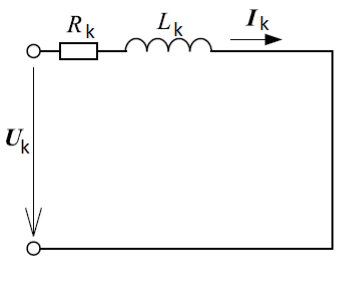
\includegraphics[width=0.5\linewidth]{ZkouskaNakratko.png}
    \caption{Zkouška nakrátko pro jednu fázi}
    \label{fig:ZkouskaNakratko}
\end{figure}

Zde jsou rovnice ze kterých jsou dopočítané hodnoty prvků nakrátko:
\begin{align}
    Rk &= \frac{P}{Ik^2*3} = \frac{40.122}{4.753^2*3} = 0.592 \Omega \\
    Zk &= \frac{Uk}{Ik} = \frac{2.821}{4.753} = 0.594 \Omega \\
    Xk &= \sqrt{Zk^2 - Rk^2} = \sqrt{0.594^2 - 0.592^2} = 0.049\Omega
    \label{eq:VypocetPrvkuNakratko}
\end{align}

Z toho jsou tedy:
\begin{itemize}
    \item Hodnoty do náhradního schématu na primáru:
    \begin{itemize}
        \item $Rk = 0.592 \Omega$
        \item $Xk = 0.049 \Omega$
    \end{itemize}
    \item Hodnoty do náhradního schématu na sekundáru:
    \begin{itemize}
        \item $Rk' = \frac{Rk}{k^2} = 24.747 m\Omega$
        \item $Xk' = \frac{Xk}{k^2} = 2.048 m\Omega$
    \end{itemize}
\end{itemize}

Hodnoty náhradních prvků na primáru ($R1 a R2'$) a sekundáru ($R1' a R2$) jsou poloviny těchto celkových rezistancí a reaktancí nakrátko. 

%%%%%%%%%%%%%%%%%%%%%%%%%%%%%%%%%%%%%%%%%%%%%%%%%%%%%%%%%%%%%%%%%%%%%%%%%%%%%%%%%%%%%%%%%%%%%%%%%%%%%%%%%%%%%%%%%%%%%%%%%%%%%%%%%%%%%%%%%%%%%%%%%%%%%%%%%%%%%%%%%%%%%%%%%%%%%%%%%%%%%%%%%%%%%%%%%%%%%%%%%%%%%%%%%%%%
\subsection{Určení velikosti prvků ze zkoušky naprázdno}
I pro zkoušku naprázdno je nejdříve nutné si přepočítat hodnotu u0 na hodnotu fázovou:
\begin{equation}
    Uk = \frac{u0}{\sqrt{3}} = \frac{8.125}{\sqrt{3}} V = 4.691 V
\end{equation}
Tohle nám dává hodnoty které jsou potřeba pro zkoušku naprázdno:
\begin{itemize}
    \item $Uo = 4.691 V$
    \item $Io = 2.432 A$
    \item $Po = 9.832 W$
\end{itemize}

Tyto hodnoty je možné dosadit do tohoto obrázku a z toho dopočítat prvky náhradního schématu, které budou vztaženy na sekundár:
\begin{figure}[H]
    \centering
    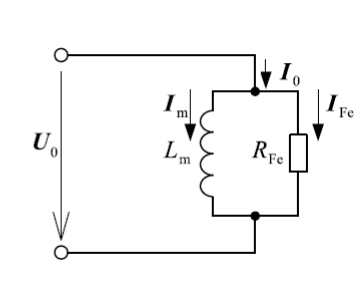
\includegraphics[width=0.5\linewidth]{ZkouskaNaprazdno.png}
    \caption{Zkouška naprázdno pro jednu fázi}
    \label{fig:ZkouskaNaprazdno}
\end{figure}

\begin{align}
    Rfe' &= \frac{Uo^2}{Po}*3 = \frac{4.691^2}{9.832}*3 = 6.714 \Omega \\
    Ife' &= \frac{Uo}{Rfe'} = \frac{4.691}{6.714} = 0.697A \\
    Im' &= \sqrt{Io^2 - Ife'^2} = \sqrt{2.432^2 - 0.697^2} = 2.330A \\
    Xm' &= \frac{Uo}{Im'} = \frac{4.691}{2.330} = 2.013 \Omega
\end{align}

Z toho jsou tedy:
\begin{itemize}
    \item Hodnoty do náhradního schématu na sekundáru:
    \begin{itemize}
        \item $Rfe' = 6.714 \Omega$
        \item $Xm' = 2.013 \Omega$
    \end{itemize}
    \item Hodnoty do náhradního schématu na primáru:
    \begin{itemize}
        \item $Rfe = k^2*Rfe' = 160.611 \Omega$
        \item $Xm = k^2*Xm' = 48.155 \Omega$
    \end{itemize}
\end{itemize}

%%%%%%%%%%%%%%%%%%%%%%%%%%%%%%%%%%%%%%%%%%%%%%%%%%%%%%%%%%%%%%%%%%%%%%%%%%%%%%%%%%%%%%%%%%%%%%%%%%%%%%%%%%%%%%%%%%%%%%%%%%%%%%%%%%%%%%%%%%%%%%%%%%%%%%%%%%%%%%%%%%%%%%%%%%%%%%%%%%%%%%%%%%%%%%%%%%%%%%%%%%%%%%%%%%%%
\section{Nakreslete dvě náhradní schémata, do jednoho vepište velikosti prvků přepočtené
na primární stranu, do druhého na sekundární.}
V této úloze vycházím z výsledků přepočtů na primár a sekundár, které proběhly v předchozím kroku hned po odvození hodnot.

Zde jsou chtěná náhradní schémata:

\begin{figure}[H]
    \centering
    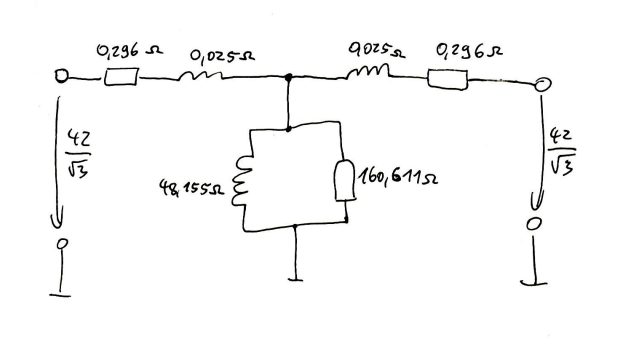
\includegraphics[width=1\linewidth]{PrepoctenoNaPrimar.png}
    \caption{Náhradní schéma přepočtené na primár}
    \label{fig:NahradniSchemaPrimar}
\end{figure}

\begin{figure}[H]
    \centering
    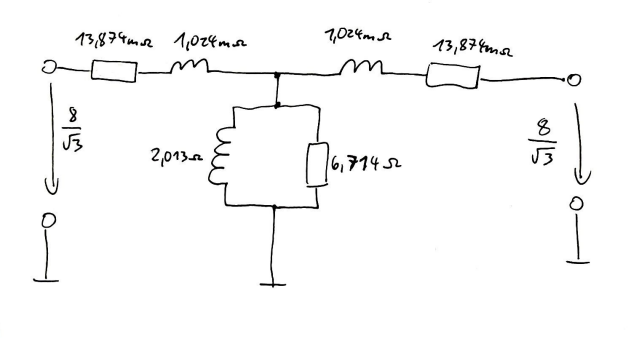
\includegraphics[width=1\linewidth]{PrepoctenoNaSekundar.png}
    \caption{Náhradní schéma přepočtené na sekundár}
    \label{fig:NahradniSchemaSekundar}
\end{figure}
%%%%%%%%%%%%%%%%%%%%%%%%%%%%%%%%%%%%%%%%%%%%%%%%%%%%%%%%%%%%%%%%%%%%%%%%%%%%%%%%%%%%%%%%%%%%%%%%%%%%%%%%%%%%%%%%%%%%%%%%%%%%%%%%%%%%%%%%%%%%%%%%%%%%%%%%%%%%%%%%%%%%%%%%%%%%%%%%%%%%%%%%%%%%%%%%%%%%%%%%%%%%%%%%%%%%
\section{Závěr}
Tohle laboratorní cvičení mělo za cíl identifikovat neznámý transformátor a tenhle cíl byl splněn.

V první části byly zjištěny odpory vinutí transformátoru, následně byl změřen a přepočítán převod, poté byly provedeny zkoušky naprázdno a nakrátko a z nich se spočítaly hodnoty prvků náhradního schématu. Nakonec byly tyto prvky náhradního schématu nakresleny všechny ve dvou náhradních schématech - jeden pro primární stranu a druhý pro sekundární stranu.

Během této identifikace jsme zjistili, že je transformátor nesymetrický a tak se při všech výpočtech počítalo s průměrnou hodnotou všech elektrických veličin jako proud, napětí a činný výkon.

Při tvoření náhradních schémat se počítalo s tím, že rezistance a reaktance změřené nakrátko jsou rovnoměrně rozděleny - tedy půl celkové změřené impedance na levé straně a půl na pravé straně.

Náhradní schémata nakreslená v poslední kapitole by se dále mohly využít pro přepočítávání primárního a sekundárního napětí v situacích, kdy je na transformátor zapojená nějaká zátěž která odebírá proud.




\end{document}